\section{MAROC chip calibration}

To allow the cross-comparison between different pixels and different MaPMTs  in universal units, and to correct for the non-linearity of the ADC readout at higher amplitudes, a procedure was developed to convert the amplitude of the MAROC slow shaper signal from ADC channels into charge. The MAROC has a built-in charge injection functionality consisting of a test input pin that is connected to the preamplifiers through a logic network of switches and 2 pF capacitors.
Together with an external step function generator, this can be used to inject a controllable amount of charge directly into the preamplifiers. We measured the output of the slow shaper in ADC channels for 82 different input charges ranging from 0 to 4 pC.
Figure~\ref{fig:MAROCcalib} shows the relationship between the injected charge and the measured amplitude in units of ADC channels for three different readout channels. The relationship between charge and ADC channels is linear up to about 1.5 pC.
This distribution was observed to vary between chips and pixels, and thus individual distributions were measured for all 64 pixels on each MAROC used in this study. 

\begin{figure}[hbt]
	\centering
	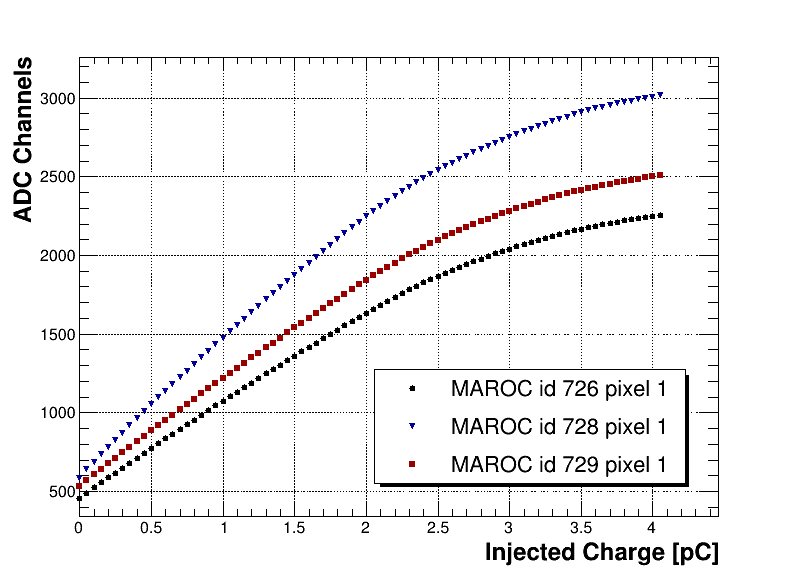
\includegraphics[width=\linewidth]{figures/adc_v_charge.png}
	\caption{Response of the MAROC slow shaper in ADC channels as a function of the injected charge. The curves shown are for pixel \#1 in three different MAROC boards.}
	\label{fig:MAROCcalib}
\end{figure}

This calibration data was used to convert the measured amplitude in ADC channels into charge collected on an event-by-event basis. A local polynomial regression was used to provide a one-to-one mapping of adc channel to charge. Figure ~\ref{fig:H12700calib} and Fig.~\ref{fig:H8500calib} show typical amplitude distributions before and after this conversion was applied for one H12700 MaPMT pixel and one H8500 MaPMT pixel, respectively. For both, the conversion to charge extends the high-amplitude tails of the spectra due to the non-linearity of the ADC readout.

\begin{figure}[hbt!]
	\centering
	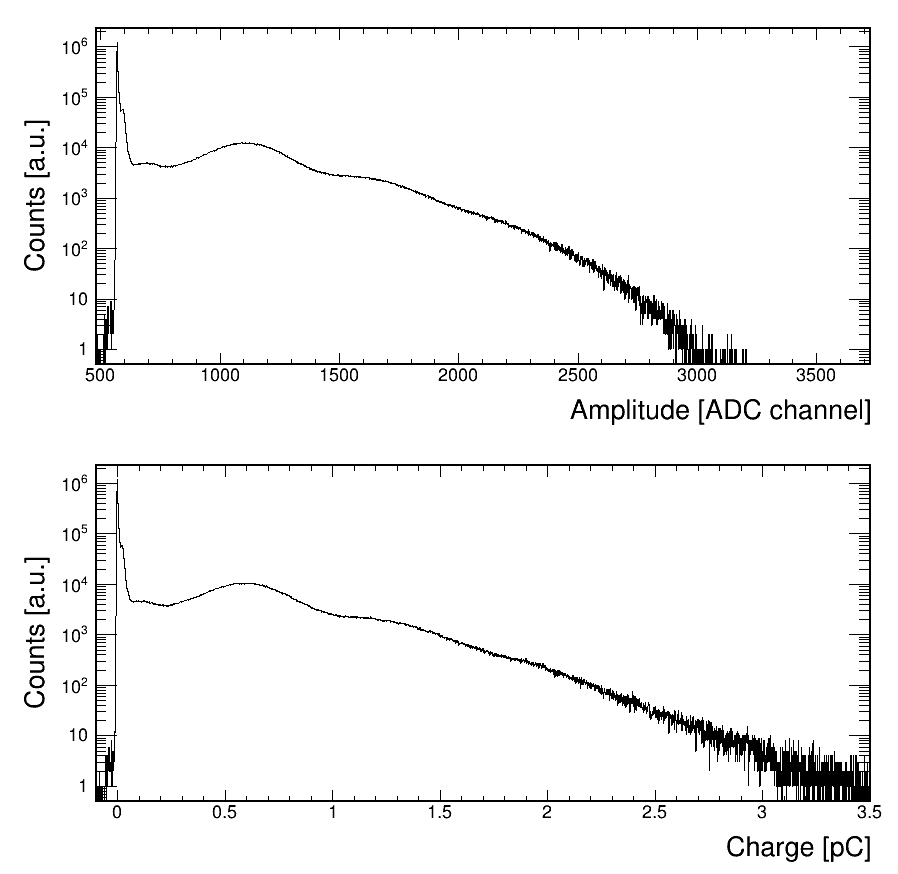
\includegraphics[width=\linewidth]{figures/GA0982_w1_g064_v1100_063_adc_charge.png}
	\caption{Top: A typical SPE spectrum for one H12700 pixel in units of ADC channel. Bottom: The same spectrum after converting the units into pC.}
	\label{fig:H12700calib}
\end{figure}

\begin{figure}[hbt!]
	\centering
	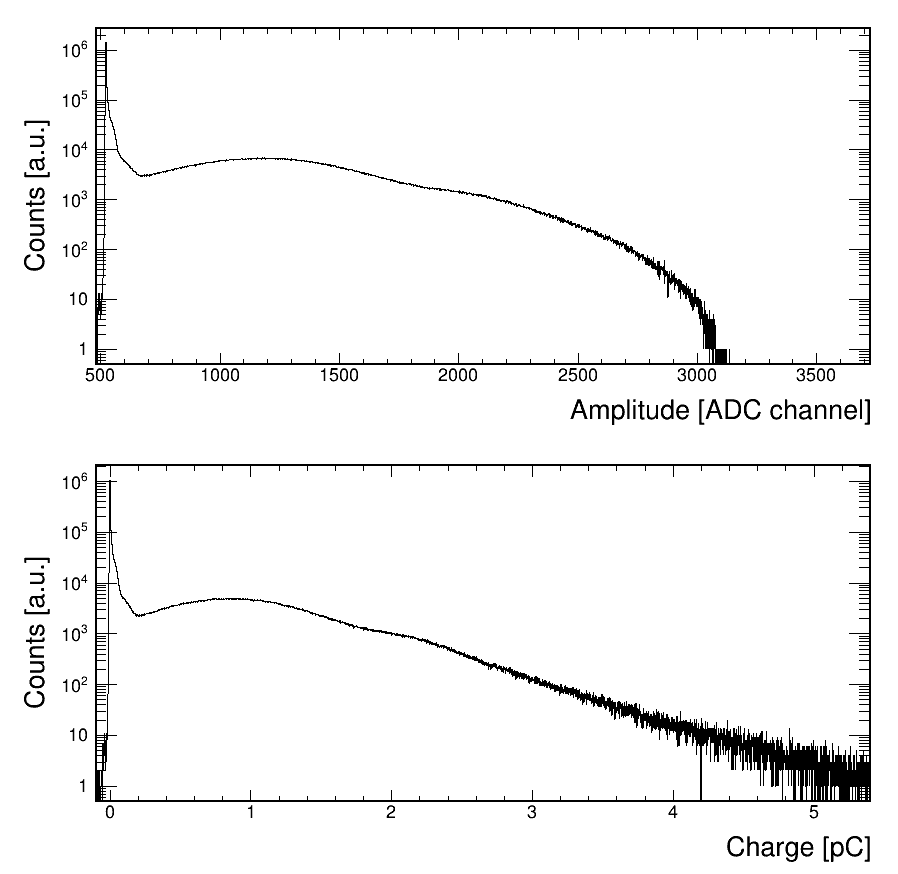
\includegraphics[width=\linewidth]{figures/CA7811_w1_g064_v1100_063_adc_charge.png}
	\caption{Top: A typical SPE spectrum for one H8500 pixel in units of ADC channels. Bottom: The same spectrum after converting the units into pC.}
	\label{fig:H8500calib}
\end{figure}
